\begin{figure*}[t]
    \centering
    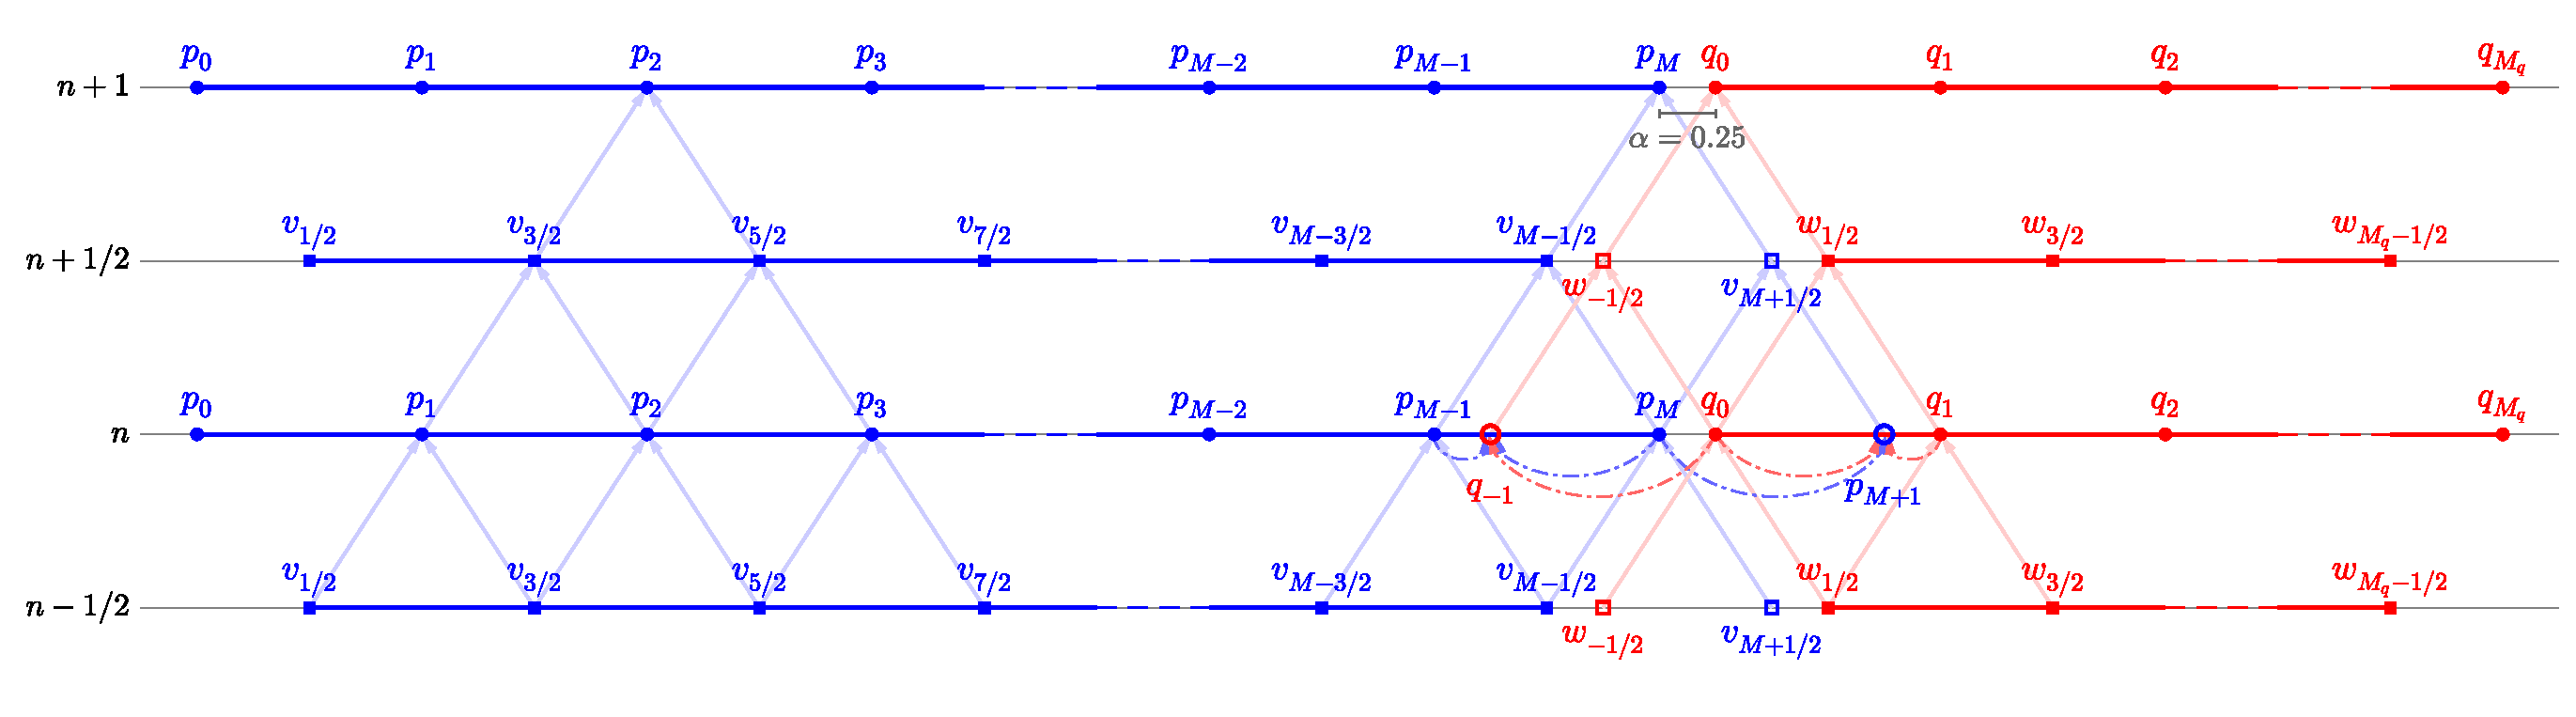
\includegraphics[width = \textwidth]{Figures/tromboneSchematic.eps}
    \caption{\it Schematic showing data flow of how different grid points at time index $n+1$ are calculated with $\alpha = 0.25$ in Eq. \eqref{eq:alphaDef}. To prevent cluttering, arrows going straight up (indicating that the state of a grid point at time step $n$ is needed to calculate the state of that grid point at $n+1$) are suppressed. As an example of the usual case, the points required to calculate $p_2^{n+1}$ are shown (refer to Eq. \eqref{eq:updateNormal}). Furthermore, the points needed to calculate $p_{M}^{n+1}$ and $q_0^{n+1}$ are shown. The most important difference with the usual case is that the virtual grid points $p_{M_p+1}^n$ and $q_{-1}^n$ 
    are the result of the interpolation of known pressure values at $n$ using Eq. \eqref{eq:connectionInterpol}. %and velocity values at $n+1/2$ respectively
    %
    %\SWcomment[Seemingly, $q_0^n$ is not calculated from anything, but it is simply $q_0^{n+1}$ time-shifted back. The same would be shown for $v_{M_p+1/2}^{n-1/2}$, but the figure does not go back-in-time more than this.]
    \label{fig:dynamicGridSchematic}}
\end{figure*}

\section{Dynamic grid}\label{sec:dynamicGrid}
The defining feature of the trombone is its slide that alters the length of the tube, changing the resonant frequencies. In a companion paper \cite{Willemsen2021}, we present a method to dynamically change grid configurations of FD schemes by inserting and deleting grid points based on an instantaneous value of the time varying wave speed $c(t)$. Although here, the tube length $L(t)$ is varied, the method still applies. %\SWcomment[So that's the thing. We're changing $c$ in the other paper, but $L$ here. Could change this to "an instantaneous value of the time varying wave speed $c(t)$. Although here, the tube length $L(t)$ is varied, the method still applies."] Though \cite{Willemsen2021} shows changes in the wavespeed $c$ rather than the length $L$, the effect of a change in either of these parameters has an identical effect on these systems \SWcomment[as long as the geometry is unchanged for the grid points.] Leaving $c$ fixed also means that grid spacing $h$ does not change during the simulation, but rather the spatial domain of the system. 
Note that this method only works for slow (sub-audio rate) parameter changes.
%\SBcomment[Not quite clear---in this paper, is it $c$ changing, or $L$? You might not need all this explanation of the equivalence between changing $c$ and $L$. ] \SWcomment[I'm changing $L$ so $c$ -- and $h$ -- are fixed. I just wanted to show that this method also works when changing another variable, but I guess the other paper already clarifies that.. Planning to remove "Though \cite{Willemsen2021} shows...spatial domain of the system." ]

We can split a tube with time-varying length $L^n$ into two smaller sections with lengths $L_p^n$ and $L_q^n$ (in m) such that $L^n = L_p^n + L_q^n$. Splitting the schemes in \eqref{eq:FDS} in this way yields two sets of first-order systems. The pressure and particle velocity of the first (left) system $p_\lp^n$ and $v_{\lp+1/2}^{n+1/2}$ are both defined over discrete domain $\lp \in \{0, \hdots, M^n\}$% \SBcomment[OK, here, don't totally get this...I would think $p$ would be defined over one more grid point than $v$, not over the same domains. This would be true for both the left hand domain and the right hand domain, assuming that $p$ lies at the subdomain endpoint.] \SWcomment[Alright, this is exactly what confused me too during this process, so let me try to explain (refer to Figure \ref{fig:dynamicGridSchematic} so it's easier to follow).. In order to calculate the inner boundaries at $n+1$ ($p_M^{n+1}$ and $q_0^{n+1}$) we need two (quadratically) interpolated points for the pressure at time-step $n$ ($p_{M+1}^n$ and $q_{-1}^n$). This is the method from \cite{Willemsen2021}. These interpolated points are used to calculate two "virtual" grid points for velocity at $n+1/2$ ($v_{M+1/2}^{n+1/2}$ and $w_{-1/2}^{n+1/2}$), which, in turn, are used to calculate $p_M^{n+1}$ and $q_0^{n+1}$. These two "virtual" velocity points I added to the discrete domains. This results in the ranges for $v$ and $w$ to be the same length as the pressure ranges $p$ and $q$. I started out by leaving them out (so $v_{\lp+1/2}^{n+1/2}$ for $\lp \in \{0, \hdots, M-1\}$ and $w_{\lq-1/2}^{n+1/2}$ for $\lq \in \{1,\hdots, M_q\}$) but for ease of working with the vectors later on it made more sense to include these in the ranges. Also we need to use the virtual velocities at $n-1/2$ ($v_{M+1/2}^{n-1/2}$ and $w_{-1/2}^{n-1/2}$) to eventually calculate $p_M^{n+1}$ and $q_0^{n+1}$ so also because of this, it made more sense to include them.] \SBcomment[Also, should $M$ be $M_{p}$ here?] \SWcomment[I left subscript $p$ out for brevity (like in the other paper there is no subscript $u$ for $M$ of the left system) as I'll use the $M$ as an index a lot later on.]
, and those of the second (right) system $q_\lq^n$ and $w_{\lq-1/2}^{n+1/2}$ are defined over discrete domain $\lq \in \{0, \hdots, M_q^n\}$, with
\begin{equation}\label{eq:MMq}
    M^n = \lceil L_p^n/h\rceil, \quad \text{and} \quad M_q^n = \lfloor L_q^n/h\rfloor
\end{equation} where $\lceil \cdot \rceil$ denotes the ceiling operation. Note, that the domains for $v$ and $w$ have an extra grid point when compared to the regular case in \eqref{eq:FDS} and that $w$ is indexed with $\lq-1/2$ rather than $\lq+1/2$. The resulting system of FD schemes then becomes
\begin{subequations}\label{eq:firstOrderPairs}
    \begin{align}
        \frac{\bar S_\lg}{\rho_0 c^2}\delta_{t+}p_\lp^n &= -\delta_{x-}(S_{\lg+1/2}v_{\lp+1/2}^{n+1/2}),\label{eq:discPressureP}\\
        \rho_0 \delta_{t-}v_{\lp+1/2}^{n+1/2}&=-\delta_{x+}p_\lp^n,\label{eq:discVelocityV}\\
        \frac{\bar S_\lg}{\rho_0 c^2}\delta_{t+}q_\lq^n &= -\delta_{x+}(S_{\lg-1/2}w_{\lq-1/2}^{n+1/2}),\label{eq:discPressureQ}\\
        \rho_0 \delta_{t-}w_{\lq-1/2}^{n+1/2}&=-\delta_{x-}q_\lq^n.\label{eq:discVelocityW}
    \end{align}
\end{subequations}
Here, due to the different indexing for $w$, the spatial derivatives for the right system are flipped. Also note, that $l$ is still used for the spatial indices of $\bar S$ and $S$ which now approximate $S(x)$ according to
\begin{equation}
S_l \approx \begin{cases}
     S(x=lh) & \text{for } x\in [0, L_p]\\
     S(x=L^n-(M_q^n-l)h) & \text{for } x\in [L_p, L]
\end{cases}
\end{equation} 
The conditions for the outer boundaries of this system, i.e., at $\lp = 0$ and $\lq = M_q^n$, are the same as for the full system. The inner boundaries, $\lp = M^n$ and $\lq = 0$ are connected according to the method described in \cite{Willemsen2021} to be explained shortly.
To be able to calculate $p_M^{n+1}$ and $q_0^{n+1}$, the domains of $v$ and $w$ have been extended at the inner boundaries to include $v_{M+1/2}^{n+1/2}$ and $w_{-1/2}^{n+1/2}$. These, however, require points outside of the domains of $p_\lp^n$ and $q_\lq^n$, i.e., $p_{M+1}^n$ and $q_{-1}^n$. In \cite{Willemsen2021} we propose to calculate these \textit{virtual grid points} based on known values of the system. Despite the fact that \cite{Willemsen2021} presents the method using a second-order system, it can still be applied here. The process of how $p_M^{n+1}$ and $q_0^{n+1}$ are calculated is visualised in in Figure \ref{fig:dynamicGridSchematic}.

\subsection{Changing the Tube Length}
In the following, the location of a grid point $u_l$ along the grid (in m from the left boundary) at time index $n$ is denoted as $x_{u_l}^n$.

The two pairs of first order systems in \eqref{eq:firstOrderPairs} are placed on the same domain $x$ with
\begin{equation}\label{eq:gridLocations}
    x_{p_\lp}^n = \lp h, \quad \text{and}\quad
    x_{q_\lq}^n = L^n-(M_q^n - \lq)h
\end{equation}
describing the locations of the left system and right system respectively. It can be observed from Eq. \eqref{eq:gridLocations} that as the tube length $L^n$ changes, the locations of the grid points of the right system will change. More specifically, as the trombone-slide is extended and $L^n$ increases, all grid points of the right system move to the right, and to the left for a contracting slide. If $L^n$ is changed in a smooth fashion, the continuous domain $x \in [0,L^n]$ will not necessarily be subdivided into an integer amount of intervals $N^n$ (of size $h = ck$). This is where a \textit{fractional} number of intervals is introduced and is defined as 
\begin{equation}\label{eq:nfrac}
    \Nfrac^n = L^n/h,
\end{equation}
which is essentially the calculation of $N$ in Eq. \eqref{eq:orderOfCalcGrid} without the flooring operation, and $N^n = \lfloor \Nfrac^n \rfloor$. The fractional part of $\Nfrac^n$ can then be calculated using
\begin{equation}\label{eq:alphaDef}
    \alpha = \alpha^n = \Nfrac^n - N^n,
\end{equation}
which describes the distance between the inner boundaries along the grid in terms of how many times $h$ would fit in-between (which is always less than once). If $\Nfrac^n = N^n$ and $\alpha = 0$, the inner boundary locations perfectly overlap, and $x_{p_M}^n = x_{q_0}^n$. This also means that the domain $x$ can be exactly divided into $N^n$ equal intervals of size $h = ck$. As the virtual grid points $p_{M+1}^n$ and $q_{-1}^n$ perfectly overlap with $q_{1}^n$ and $p_{M-1}^n$ respectively, these values can be used directly to calculate the inner boundaries. This situation effectively acts as a rigid connection between the inner boundaries defined as
\begin{equation}\label{eq:rigidConn}
    p_M^n = q_0^n, \quad \text{if} \ \  \alpha = 0.
\end{equation}
%
If $\alpha \neq 0$, some other definition for $p_{M+1}^n$ and $q_{-1}^n$ needs to be found. We use quadratic Lagrangian interpolation according to
\begin{subequations}\label{eq:connectionInterpol}
\begin{align}
        &p_{M+1}^n = \frac{\alpha - 1}{\alpha + 1}p_{M}^n + q_0^n - \frac{\alpha - 1}{\alpha + 1}q_1^n,
    \label{eq:calcPMp1}\\
        &q_{-1}^n
        =-\frac{\alpha - 1}{\alpha + 1}p_{M-1}^n + p_{M}^n+ \frac{\alpha - 1}{\alpha + 1}q_{0}^n\label{eq:calcQm1},
\end{align}
\end{subequations}
which can then be used to calculate $v_{M+1/2}^{n+1/2}$ and $w_{-1/2}^{n+1/2}$ and consequently $p_M^{n+1}$ and $q_0^{n+1}$. This process repeats every sample. It can be shown through the rigid connection in \eqref{eq:rigidConn}, that if $\alpha=0$, the definitions in \eqref{eq:connectionInterpol} reduce to $p_{M+1}^n = q_1^n$ and $q_{-1}^n = p_{M-1}^n$ as stated before.

\subsection{Adding and removing grid points}\label{sec:addRemove}
As the tube length $L^n$ changes, $L_p^n$ and $L_q^n$ also change according to
\begin{equation}
    L_p^n = L_p^{n-1} + 0.5 L_\text{diff}^n, \quad L_q^n =  L_q^{n-1} + 0.5L_\text{diff}^n,\label{eq:updateLs} 
\end{equation}
where
\begin{equation}
    L_\text{diff}^n = L^n-L^{n-1},\label{eq:lDiff}
\end{equation}
which causes the number of points $M^n$ and $M_q^n$ to change as well, according to Eq. \eqref{eq:MMq}.

The following state vectors are introduced for the pressure, defined for $n+1$ and $n$ %\SWcomment[($n-1$ is used later on for the state correction, say something about that here or leave for Section \ref{sec:impStateCorr}..?)]
\begin{equation}
    \mathbf{p}^n = [p_0^n, p_1^n, ..., p_M^n]^T,\ \mathbf{q}^n = [q_0^n, q_1^n, ..., q_{M_q}^n]^T
\end{equation}
and for the velocity, defined for $n+1/2$ and $n-1/2$
\begin{equation}
    \begin{aligned}
        \mathbf{v}^{n-1/2} &=  [v_{1/2}^{n-1/2}, v_{3/2}^{n-1/2}, ..., v_{M+1/2}^{n-1/2}]^T\\
        \mathbf{w}^{n-1/2} &=  [w_{-1/2}^{n-1/2}, w_{1/2}^{n-1/2}, ..., w_{M_q-1/2}^{n-1/2}]^T
    \end{aligned}
\end{equation}
and contain the different states over the discrete domains defined at the beginning of this section. Here, $T$ denotes the transpose operation.

If $N^n>N^{n-1}$, points are added to the left and right system in an alternating fashion %\SWcomment[(same here for $n-1$ in the state correction, say something about that here or leave for Section \ref{sec:impStateCorr}..?)]
\begin{equation}\label{eq:addingPoint}
    \begin{aligned}
        \!\!\!\!\!&\begin{cases}
            \mathbf{p}^n = [(\mathbf{p}^n)^T, I_3\mathbf{r}^n]^T\\
            \mathbf{v}^{n-1/2} = [(\mathbf{v}^{n-1/2})^T, I_3\mathbf{z}_v^{n-1/2}]^T
        \end{cases}
        \quad\!\text{if $N^n $ is odd},\\
        \!\!\!\!\!&\begin{cases}
            \mathbf{q}^n = [I_3^\flip\mathbf{r}^n, (\mathbf{q}^n)^T]^T\\
            \mathbf{w}^{n-1/2} = [ I_3^\flip\mathbf{z}_w^{n-1/2},(\mathbf{w}^{n-1/2})^T]^T
        \end{cases}\text{if $ N^n$ is even},
    \end{aligned}
\end{equation}
where
\begin{equation}\label{eq:interpVecs}
    \begin{aligned}
        \!\!\!\!\mathbf{r}^n &= [p_{M-1}^n, p_M^n, q_0^n, q_1^n]^T,\\
        \!\!\!\!\mathbf{z}_v^{n-1/2} &= [v_{M-1/2}^{n-1/2}, v_{M+1/2}^{n-1/2}, w_{1/2}^{n-1/2}, w_{3/2}^{n-1/2}]^T - \boldsymbol{\eta},\\
        \!\!\!\!\mathbf{z}_w^{n-1/2} &= [v_{M-3/2}^{n-1/2}, v_{M-1/2}^{n-1/2}, w_{-1/2}^{n-1/2}, w_{1/2}^{n-1/2}]^T+ \boldsymbol{\eta}^{\flip},% \quad\text{and}\\
        %     \mathbf{v}_\star^n &= [w_1^n, w_0^n, u_M^n, u_{M-1}^n],
    \end{aligned}
\end{equation}
cubic Lagrangian interpolator
\begin{equation}\label{eq:customIp}
    I_3 = \begin{bmatrix} -\frac{\alpha(\alpha+1)}{(\alpha+2)(\alpha+3)} &\frac{2\alpha}{\alpha+2} &\frac{2}{\alpha+2} 
    &-\frac{2\alpha}{(\alpha+3)(\alpha+2)}
    \end{bmatrix},
\end{equation}
and 
\begin{equation}\label{eq:offsetVec}
    \boldsymbol{\eta} = \boldsymbol{\eta}^{n-1/2}= \left(w_{-1/2}^{n-1/2}-v_{M+1/2}^{n
    -1/2}\right)\cdot[0, 0, 1, 1]^T 
\end{equation}
adds an offset to half of the $\mathbf{z}$ vectors depending on the difference between $v_{M+1/2}^{n-1/2}$ and $w_{-1/2}^{n-1/2}$. Why this is necessary will be further explained in Section \ref{sec:drift}. Finally, $I_3^\flip$ and $\boldsymbol{\eta}^{\flip}$ are flipped versions of \eqref{eq:customIp} and \eqref{eq:offsetVec} respectively.

If $N^n < N^{n-1}$, points are simply removed from the vectors according to

\begin{equation}\label{eq:removingPoint}
    \begin{aligned}
        &\begin{cases}
            \mathbf{p}^n = [p_0^n, \hdots, p_{M-1}^n]^T\\
            \mathbf{v}^{n-1/2} = [v_{1/2}^{n-1/2}, \hdots, v_{M-1/2}^{n-1/2}]^T
        \end{cases}
        \quad\!\text{if $N^n$ is even},\\
        &\begin{cases}
            \mathbf{q}^n = [q_1^n, \hdots, q_{M_q}^n]^T\\
            \mathbf{w}^{n-1/2} = [w_{1/2}^{n-1/2},\hdots, w_{M_q-1/2}^{n-1/2}]^T
        \end{cases}\text{if $ N^n$ is odd}.
    \end{aligned}
\end{equation}
Notice that the even and odd conditions in Eqs. \eqref{eq:addingPoint} and \eqref{eq:removingPoint} can be swapped. To stay as close to the desired location of adding and  removing grid points as possible, this requires the ceiling and flooring operations in \eqref{eq:MMq} to be swapped as well.
\subsection{Drift of $w$}\label{sec:drift}
The inner boundaries of the pressure states $p$ and $q$ are connected by \eqref{eq:connectionInterpol}, but no such connection exists for the velocity states $v$ and $w$. As the radiating boundary is implemented on the pressure grid, \SWcomment[$\leftarrow$ what about this for the explanation of the drift?] this leaves $w$ without any boundary condition; it is only ``held in place'' by the pressure values of $q$, or more specifically, by derivatives (both spatial and temporal). As FD schemes are an approximation, it does not give a perfect solution and $w$ tends to `drift' during the simulation, especially when $L^n$ is changed.

Luckily, as the pressure values are also calculated from derivatives of the velocity, the absolute state of $w$ does not matter. The difference in values at the connection point is also irrelevant as there is no spatial derivative taken between $v$ and $w$ (refer to Figure \ref{fig:dynamicGridSchematic}). Finally, the pressure values are used for the output audio of the simulation, so the drift does not cause any audible artefacts. 

The absolute states of the velocity vectors do, however, need to be accounted for when adding points to the $\mathbf{v}$ and $\mathbf{w}$ using \eqref{eq:addingPoint}. The current drift can be approximated by observing the difference between $w_{-1/2}^{n-1/2}$ and $v_{M+1/2}^{n-1/2}$, as these have approximately the same $x$ location ($x_{w_{-1/2}}^n \approx x_{v_{M+1/2}}^n$) when a grid point is added. This is then used in a drift-correction vector $\boldsymbol{\eta}^{n-1/2}$ presented in \eqref{eq:offsetVec}. When a point is added to $v$, the values of $w$ in $\mathbf{z}_{v}$ are offset by the aforementioned difference and when a point is added to $w$ the same happens (inverted) for the values of $v$ in $\mathbf{z}_w$. This way, the drift is allowed, but does not affect the state of the newly added grid points. Notice that the drift does not affect the operations of point removal in \eqref{eq:removingPoint}.

\subsection{State Correction}
As $L^n$, and consequently the number of grid points, is decreased, it might occur that the inner boundaries $p_M^n$ and $q_0^n$ have a very different value when $\alpha \gtrsim 0$, i.e., right before a point is removed. This violates the rigid connection in Eq. \eqref{eq:rigidConn}. 

We propose in \cite{Willemsen2021} to add an artificial spring-like connection between the inner boundaries that ``corrects'' the state of these points. Applying this to system \eqref{eq:firstOrderPairs} extends Eqs. \eqref{eq:discPressureP} and \eqref{eq:discPressureQ} according to
\begin{subequations}\label{eq:pressuresWithSC}
    \begin{align}
        \frac{\bar S_\lg}{\rho_0 c^2}\delta_{t+}p_\lp^n &= -\delta_{x-}(S_{\lg+1/2}v_{\lp+1/2}^{n+1/2}) + J_p(x_{p_M}^n)F_\text{sc}^n\label{eq:pWithSC}\\
        \frac{\bar S_\lg}{\rho_0 c^2}\delta_{t+}q_\lq^n &= -\delta_{x+}(S_{\lg-1/2}w_{\lq-1/2}^{n+1/2}) - J_q(x_{q_0}^n)F_\text{sc}^n\label{eq:qWithSC}
    \end{align}
\end{subequations}
where spreading operators
\begin{equation}\label{eq:spreadingOperators}
    \begin{aligned}
    J_p(x_i^n)& =
    \begin{cases}
        \frac{1}{h}, & \lp = \lp_{\!,i} = \lfloor x_i^n/h\rfloor\\
        0,& \text{otherwise},
    \end{cases}
    \quad\text{and}\\
    J_q(x_i^n) &=
    \begin{cases}
        \frac{1}{h}, & \lq = \lq_{\!,i} = \lfloor x_i^n/h \rfloor - M^n\\
        0,& \text{otherwise}.
    \end{cases}
\end{aligned}
\end{equation}
\SWcomment[should $\lp_{,i}$ and $\lq_{,i}$ also get a $n$ superscript?]Furthermore, correction effect
\begin{equation}\label{eq:scForce}
    F_\text{sc}^n = \beta\left(\mu_{t\cdot}\eta_\text{sc}^n+\sigma_\text{sc}\delta_{t\cdot}\eta_\text{sc}^n\right),
\end{equation}
% (in m$^{3}$/s)\SWcomment[..units stop making sense here as this is an artificial connection ``force''.. might just exclude them?]
with spring damping $\sigma_\text{sc}$, pressure difference
\begin{equation}
    \eta_\text{sc}^n \triangleq q_0^n - p_M^n
\end{equation} 
and scaling coefficient
\begin{equation}\label{eq:betaDef}
    \beta = \beta(\alpha) = \frac{1-\alpha}{\alpha+\epsilon},
\end{equation}
where $\epsilon\ll 1$ to prevent division by 0. Just like in \cite{Willemsen2021}, implementing the pressure difference allows for an infinite $\beta$ ($\epsilon = 0$) acting like a rigid connection between Eqs. \eqref{eq:pWithSC} and \eqref{eq:qWithSC}.
% One can write the entire system above in matrix form by concatenating...
